\section{Gradient peak}\label{sec:gradient-peak}
In~\cite{Hammer-2021} their input perturbation visualization technique did not show the expected effect of modulations in the high-gamma frequency bands on the network's predictions.
While studying it further using a different visualization technique, namely the gradient visualization (see Section~\ref{subsec:gradinet-visualization}), they found that this visualization technique also does not show any interest of the CNNs in the high-gamma frequency band, unless the input window is shortened so that the CNN has only one output, i.e. predicts one time-point.

Two interesting observations can be made when we visualize gradients of a Deep4Net which makes one prediction:
\begin{enumerate}
\item A gradient peak occurs at 83.88~Hz in both the untrained and the trained network and it is amplified with training.
\item If we add noise of a certain frequency or white noise to the input, frequencies around 83.33~Hz increase in the output of the network, compared to the original output.
\end{enumerate}

A hypothesis was that the 83.33~Hz peak occurs due to this frequency being aligned with the dilations of the max-pool layers and therefore is just an architecture artifact.
Because the sampling rate is 250~Hz and the dilations of the max-pool layers are powers of three and $250 Hz / 3 = 83.33 Hz$, this frequency aligns with the dilations of the max-pool layers which amplify it.
However, this does not explain why the peak at 83.33~Hz increases with training.

To test the artifact hypothesis, we systematically changed the dilations of the max-pool layers to powers of 1, 2 and 3 and kernel sizes to 1\footnote{Importantly, a max-pool layer with kernel size one is equivalent to no max-pool layer. Therefore, if all max-pool layers in a DNN have their kernel size set to 1, it is equivalent to a  without max-pool layers.}, 2, 3 and 4. For an overview of the tested architectures see Table \ref{tab:architectures-description}.

The results in Figure~\ref{fig:gradient-peak} demonstrate that the kernel size change has no effect on the 83.33~Hz peak.
However, with change in the dilations, the 83.33~Hz peak disappears without.
The disappearance has no effect on the performance of the network. 
It is also interesting to observe how the gradients of motor, non-motor and all channels behave with respect to each other for different frequencies.
The biggest differences between the gradients are in the alpha and beta bend where the motor gradients have visibly higher values than non-motor and all channels.
For the gradient peak at 83.33~Hz, the values of the motor, non-motor and all channels are almost equivalent. \\

\begin{figure}
\begin{subfigure}{\textwidth}
  \centering
  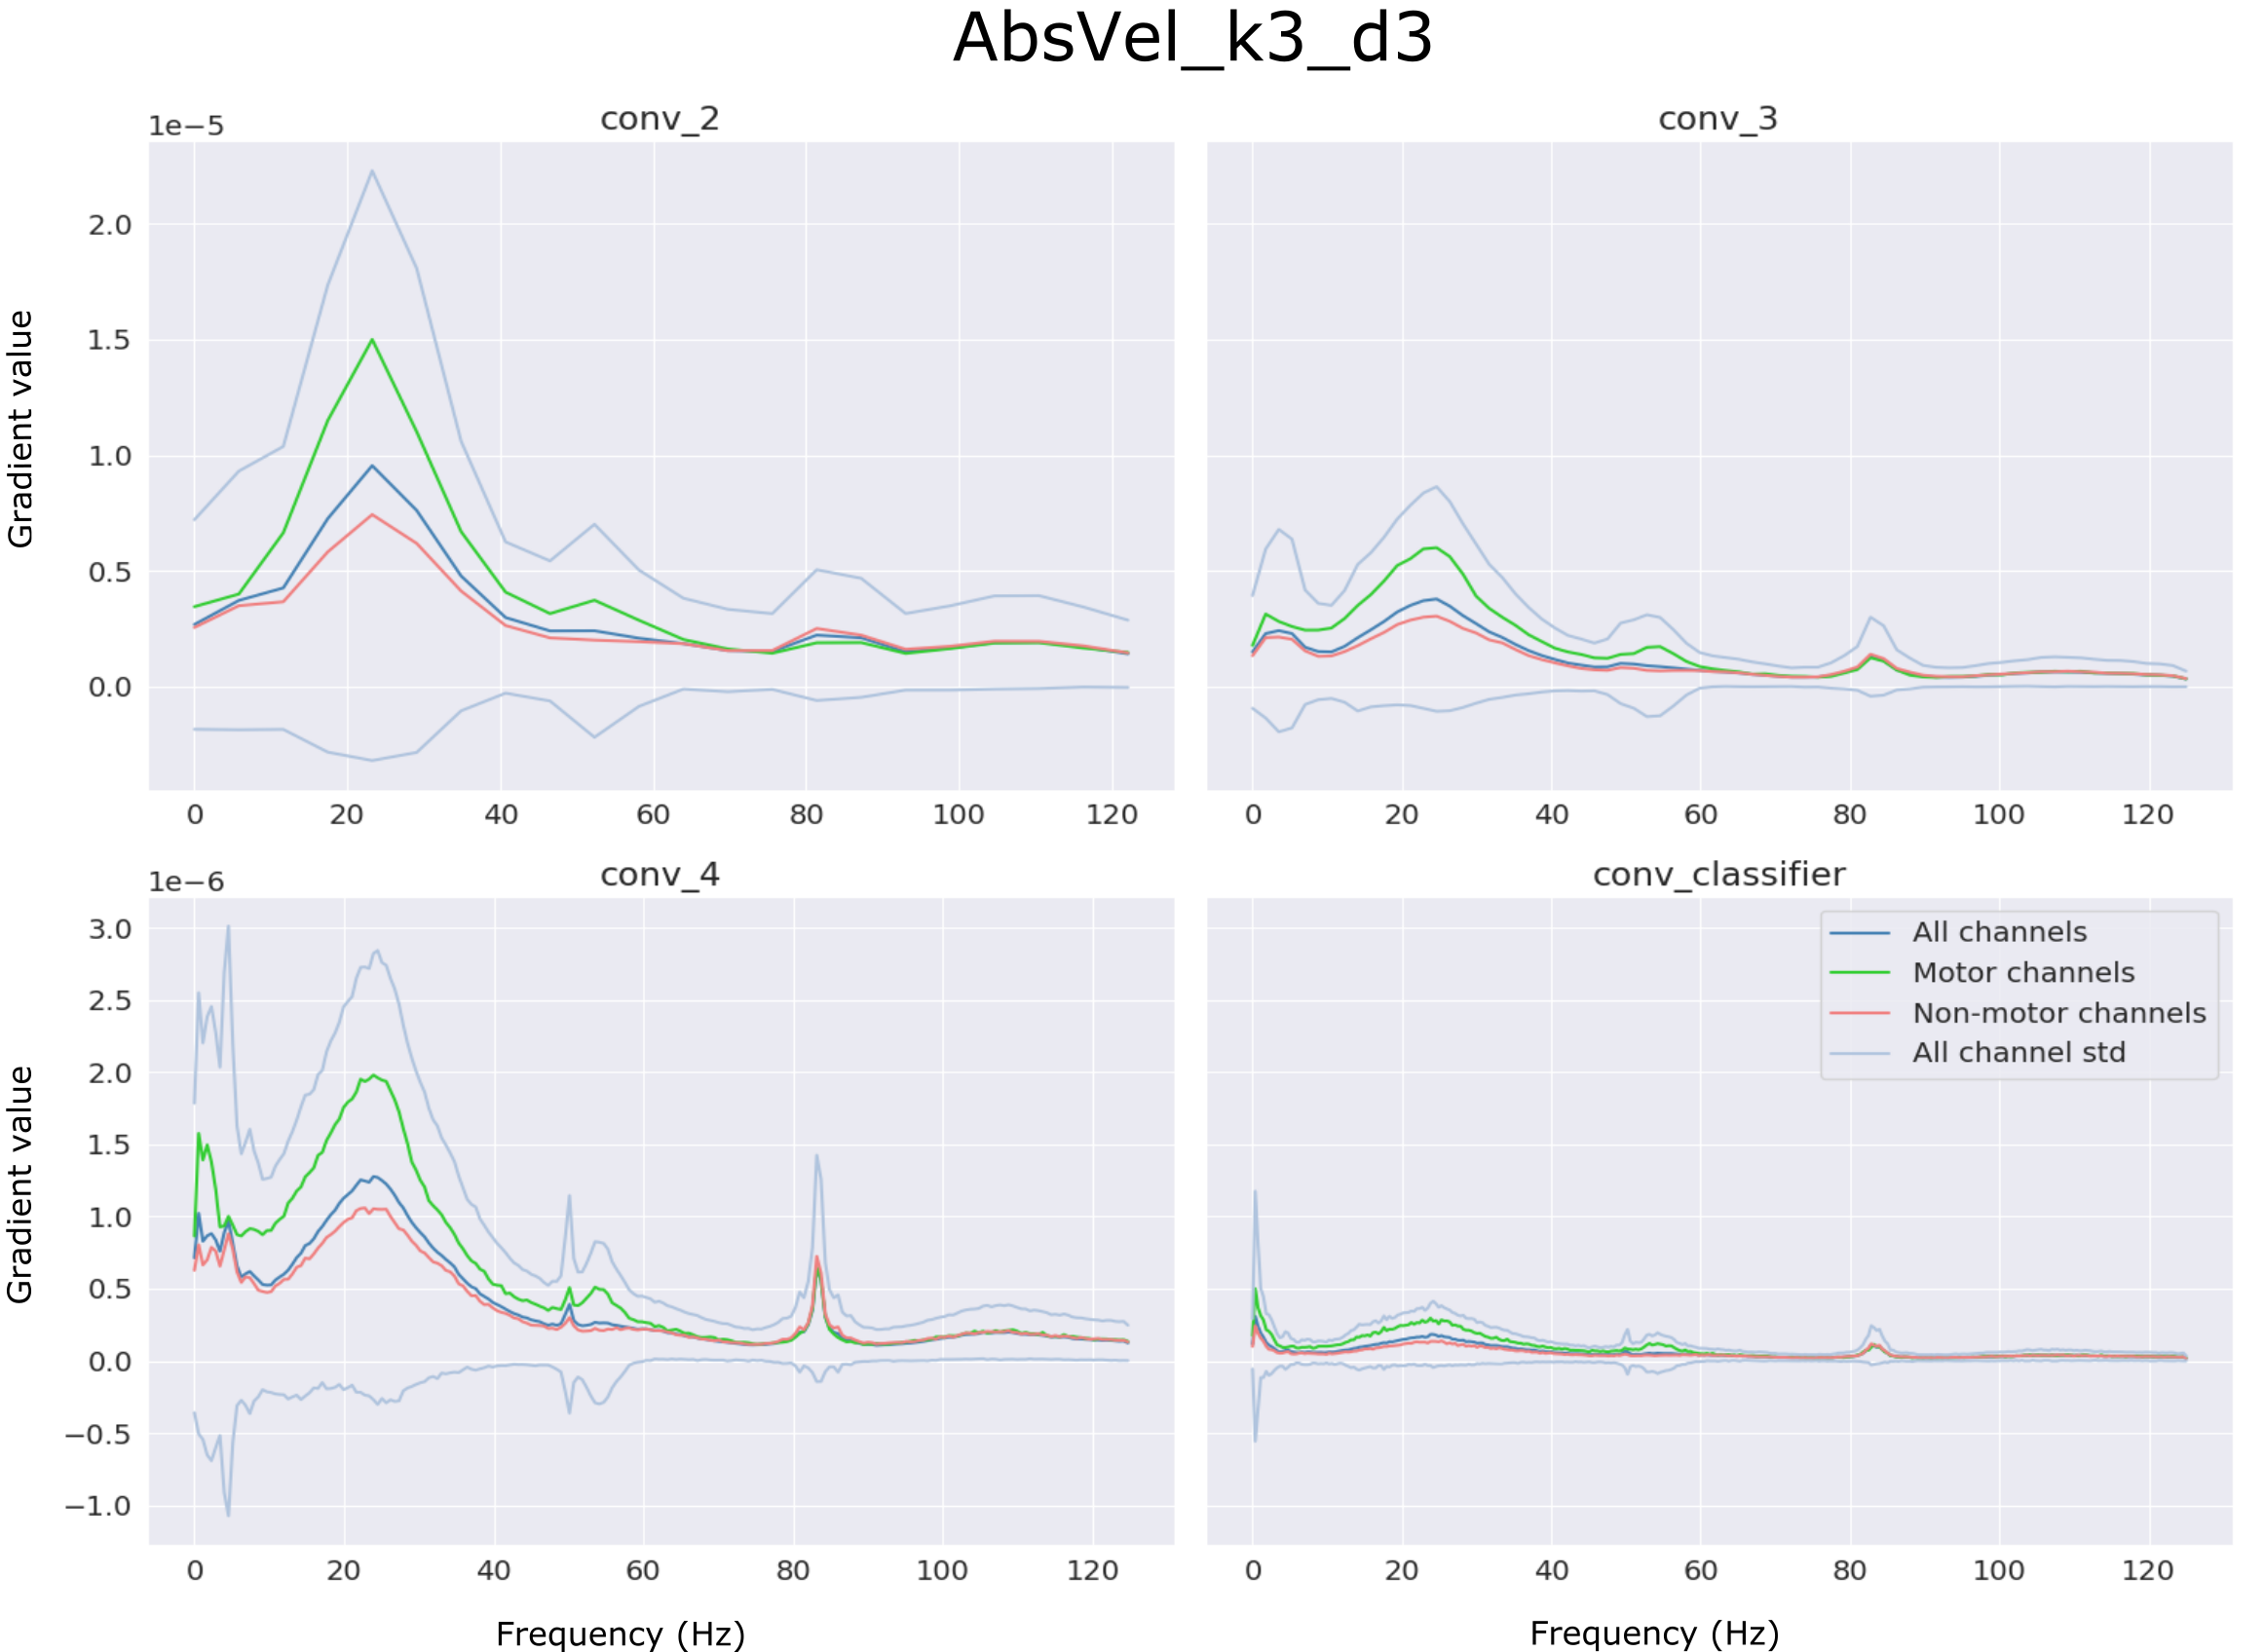
\includegraphics[width=0.6\linewidth]{img/ch4/absVel-k3-d3}
  \caption{1a}
  \label{fig:absVel-k3-d3}
\end{subfigure}%
\\
\begin{subfigure}{\textwidth}
  \centering
  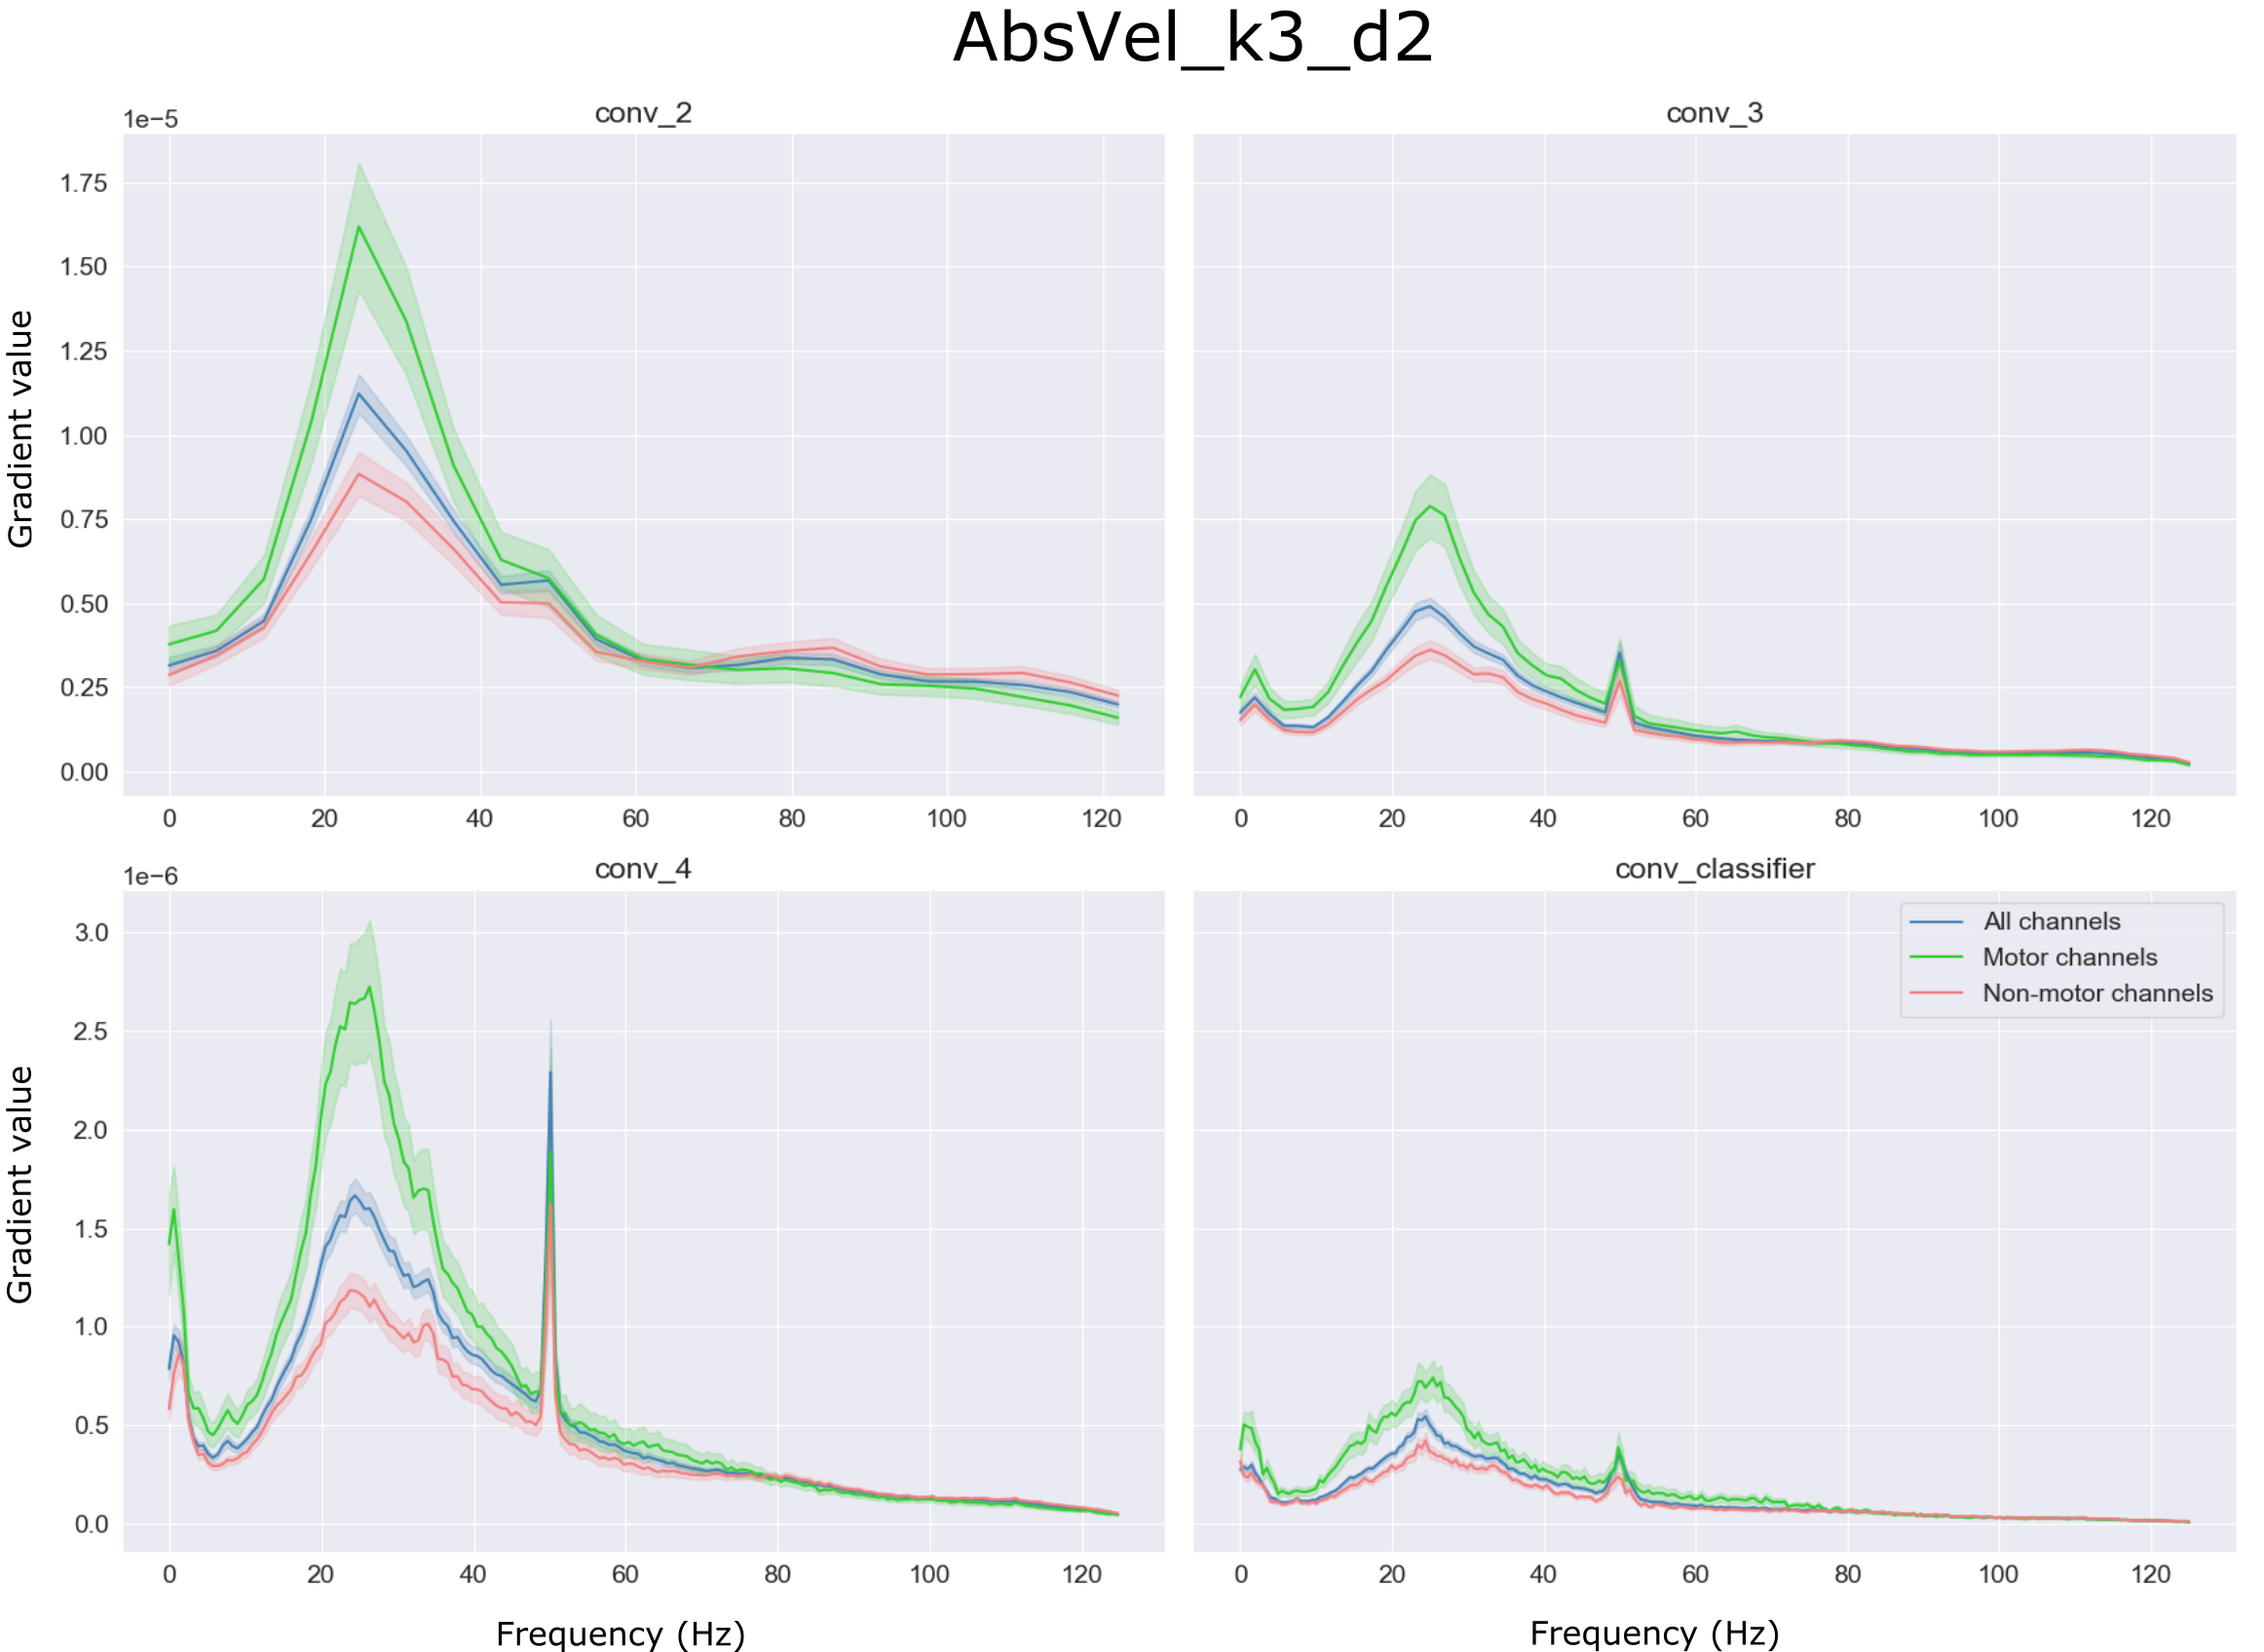
\includegraphics[width=0.6\linewidth]{img/ch4/absVel-k3-d2}
  \caption{}
  \label{fig:absVel-k3-d2}
\end{subfigure}
\begin{subfigure}{\textwidth}
  \centering
  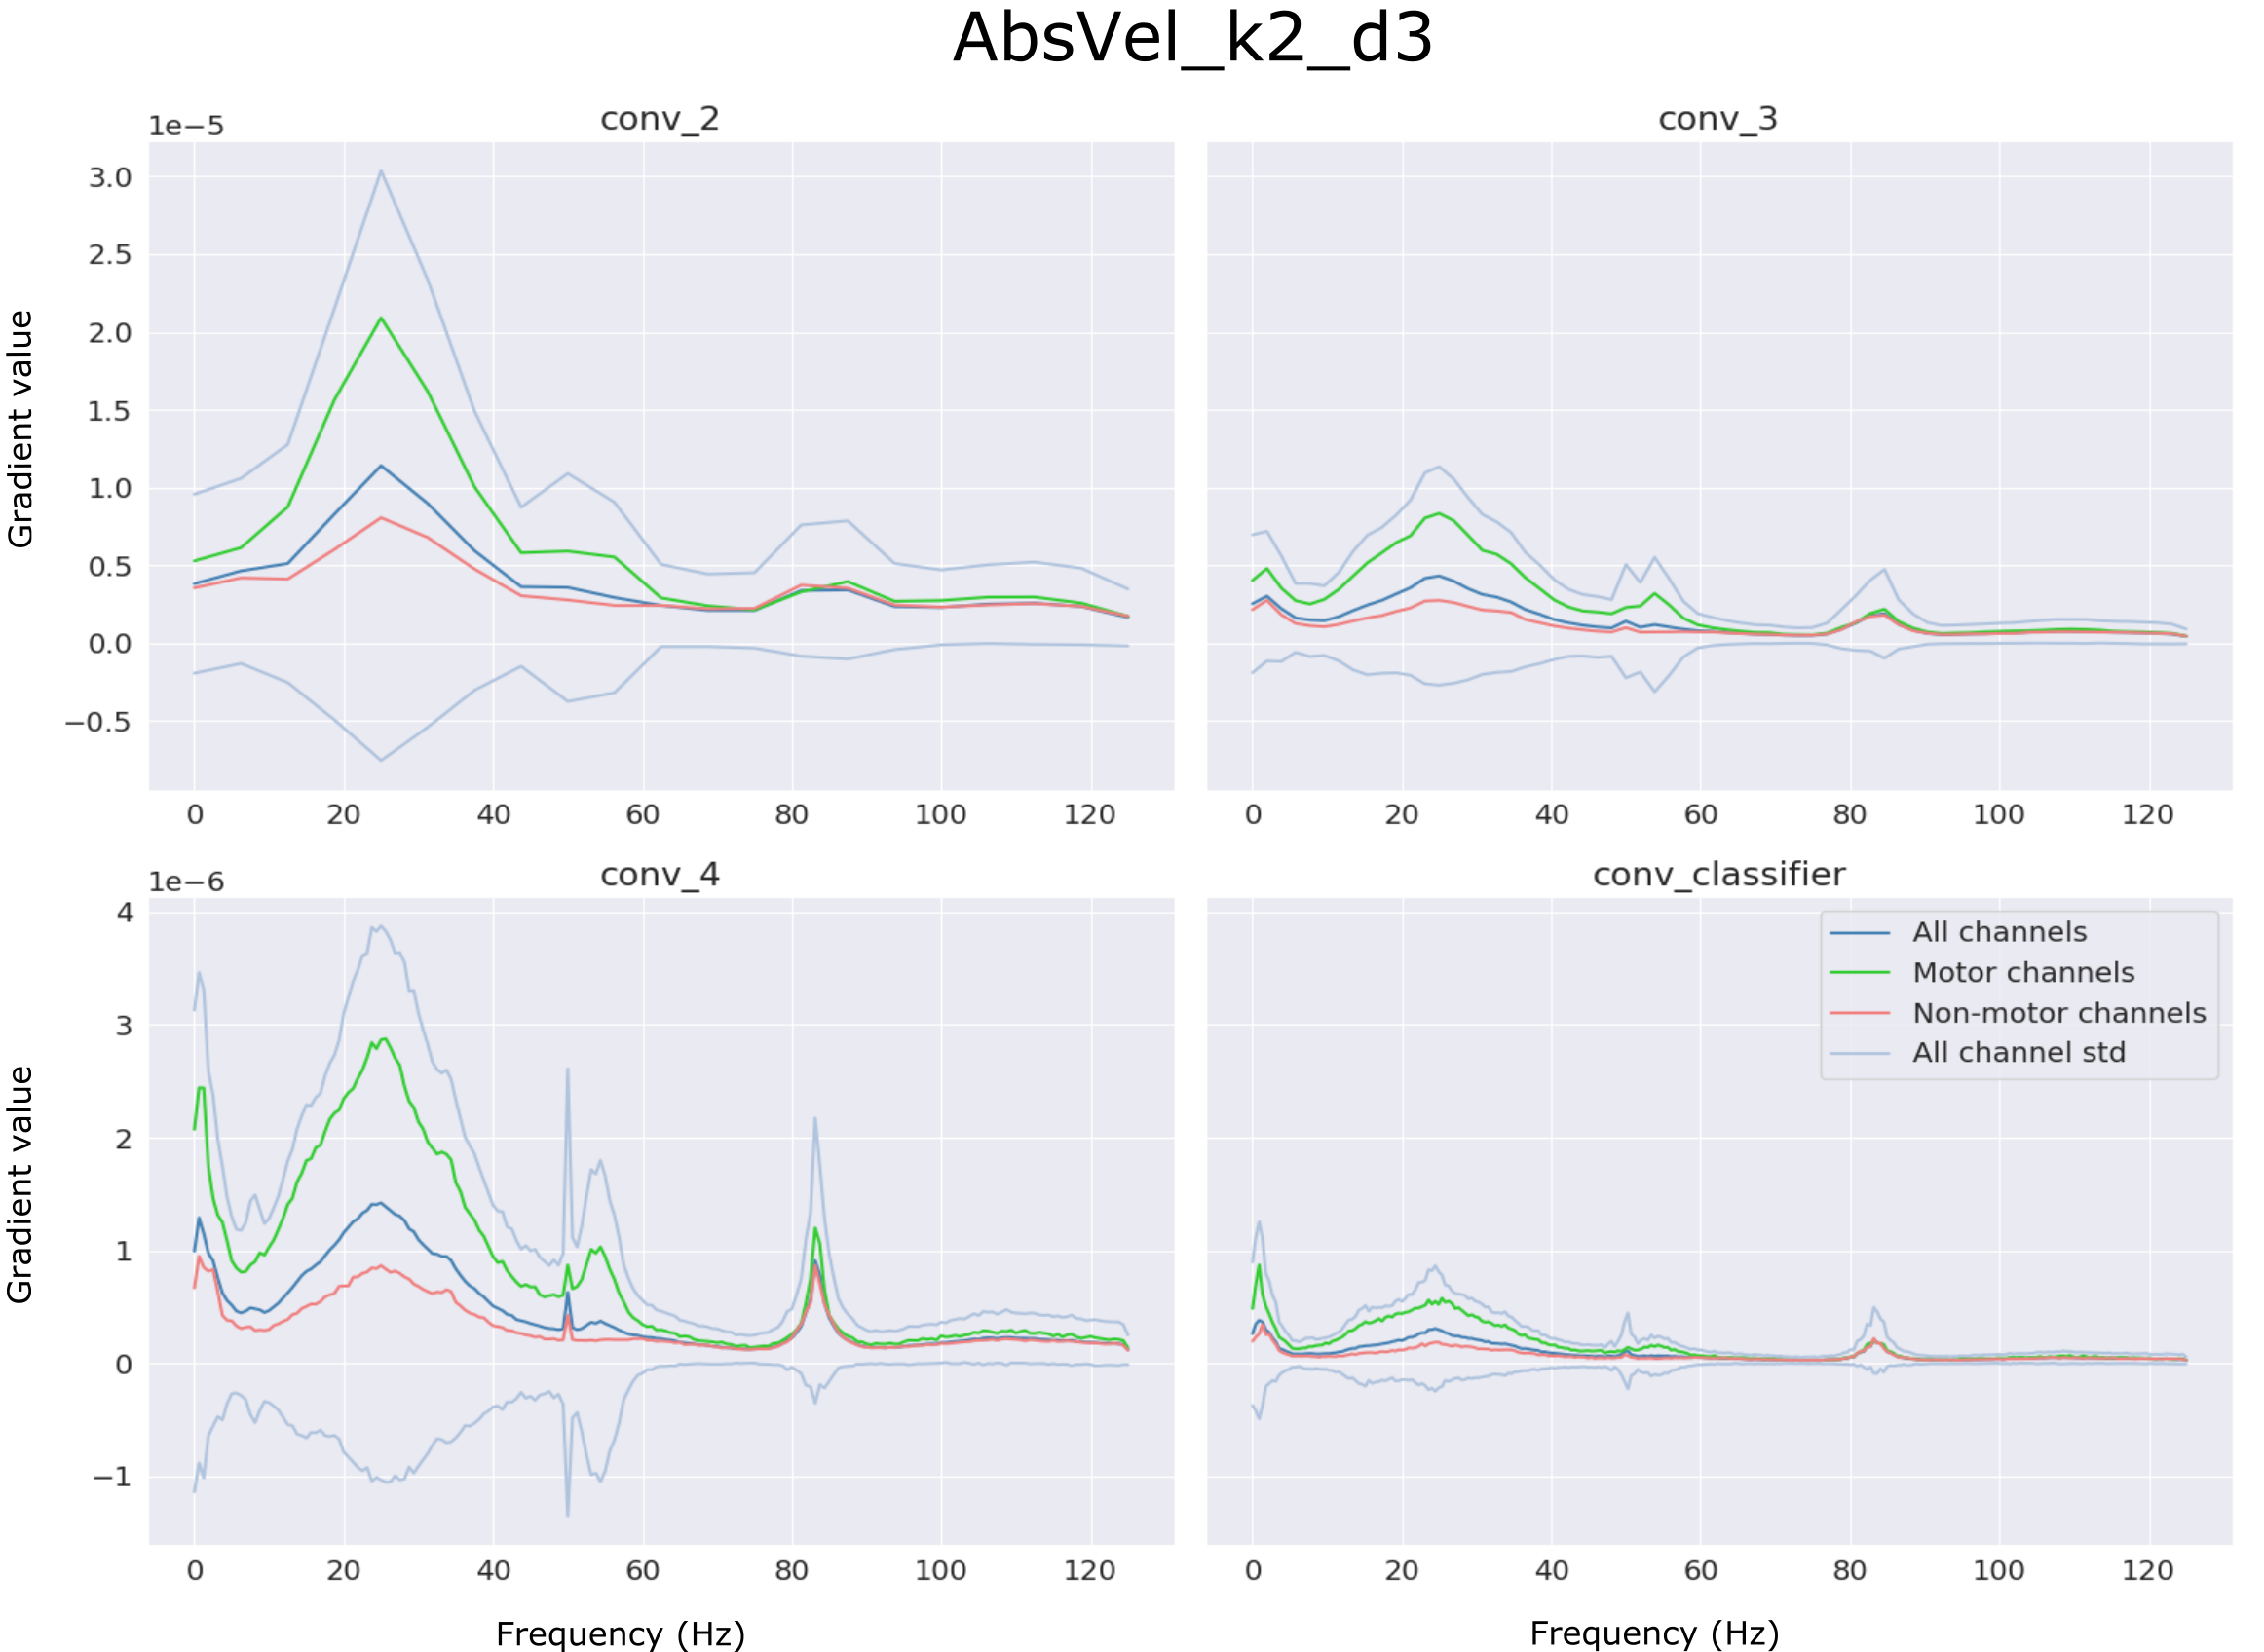
\includegraphics[width=0.6\linewidth]{img/ch4/absVel-k2-d3}
  \caption{1a}
  \label{fig:absVel-k2-d3}
\end{subfigure}
\caption{Gradients of intermediate layers of CNNs decoding absolute velocity. The displayed networks are \textbf{(a)} the Deep4Net with stride before pool True (k3\_d3\_sbp1); \textbf{(b)} k3\_d2 meaning, the kernel sizes stayed unchanged and the dilations were altered to powers of two; \textbf{(c)} k2\_d3 meaning, the kernel sizes were altered and the dilations stayed the same as for the Deep4Net.}
\label{fig:gradient-peak}
\end{figure}

The increase of the 83.33~Hz frequency in the output also vanished when changing the dilations of the max-pool layers.
To study specifically, how the dilations in the max-pool layers affect the increase of the 83.33~Hz frequency in the output, we studied how the signal itself is affected by max-pool layers only.
We used one and four max-pool layers with dilations equivalent with those from the Deep4Net (k3\_d3\_sbp1).
The result for one max-pool layer is presented in Figure~\ref{fig:max-pool-changes}
When the max-pool layer dilation parameter is three (or powers of three in the case of multiple consecutive max-pool layers), the output signal exhibits periodical peaks with the greatest peak around 83.33~Hz \ref{fig:maxpool-k3-d3}.
When the dilation of the max-pool layers are set to two and powers of two, the periodicity of the peaks still occurred, however, the period increased and the greatest peak was around 0 and 120~Hz \ref{fig:maxpool-k3-d2}.
This is in line with the hypothesis that the alignment of frequencies with the max-pool layer dilations is indeed the reason for the increase of this frequency in the output. \\


\begin{figure}
\centering
\begin{subfigure}[b]{\textwidth}
   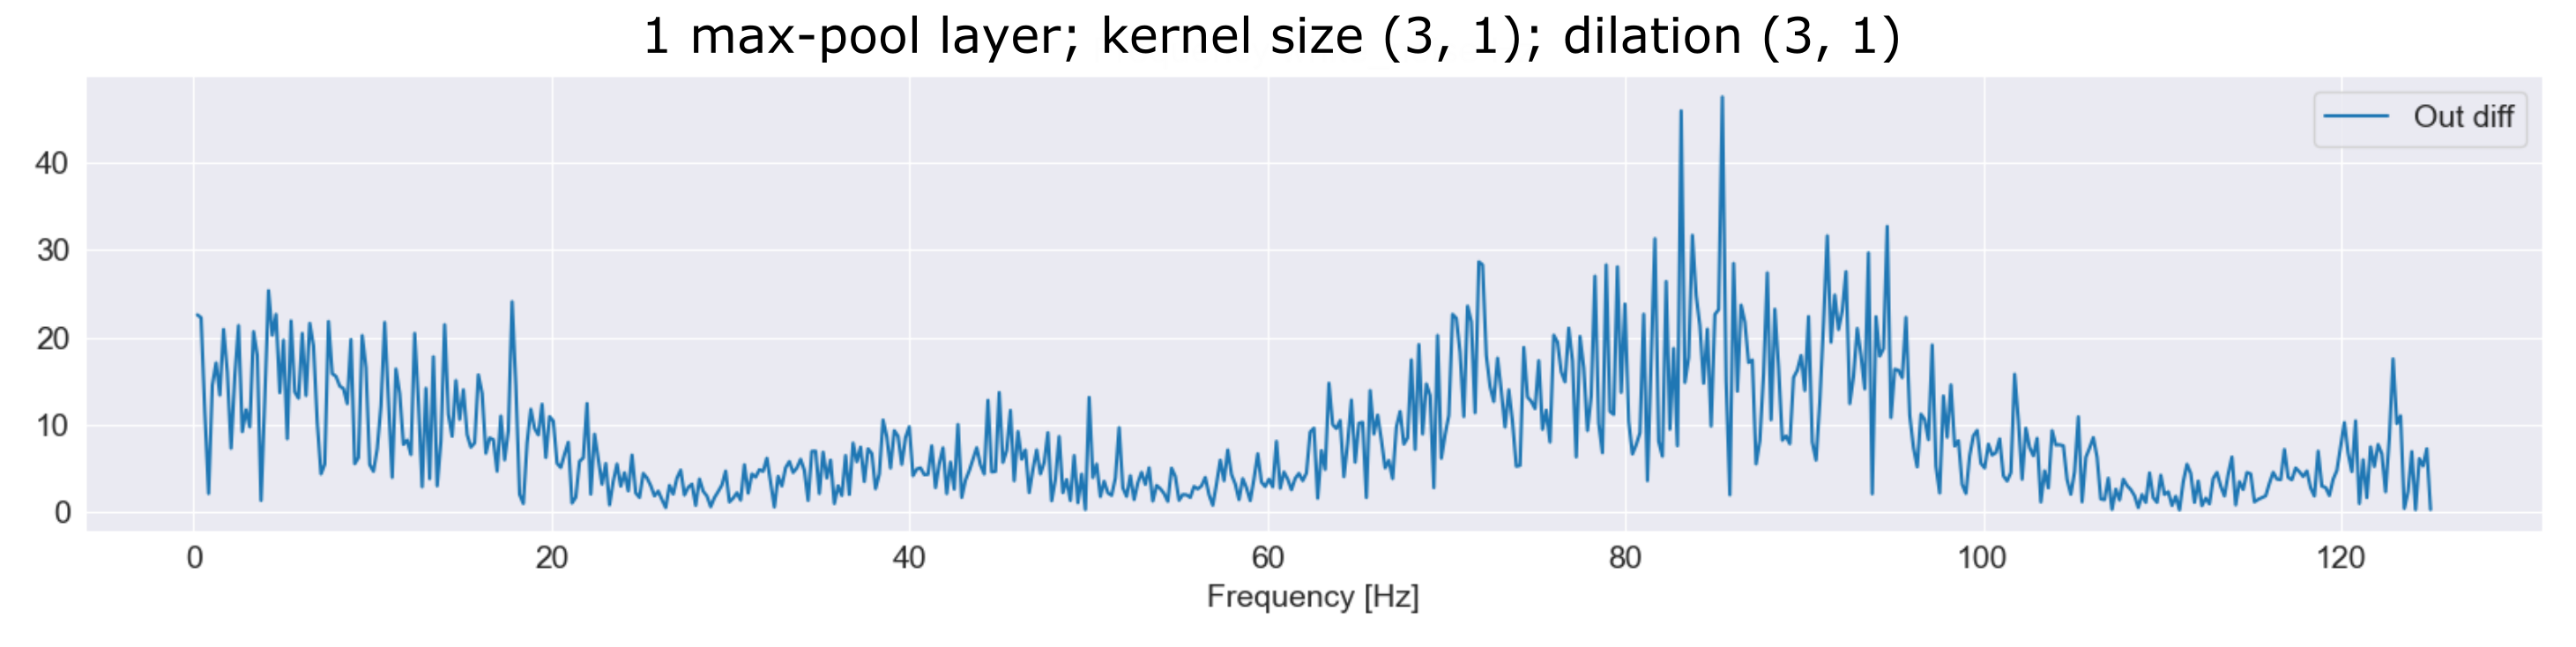
\includegraphics[width=1\linewidth]{img/ch4/absVel-maxpool-k3-d3}
   \caption{}
   \label{fig:maxpool-k3-d3} 
\end{subfigure}

\begin{subfigure}[b]{\textwidth}
   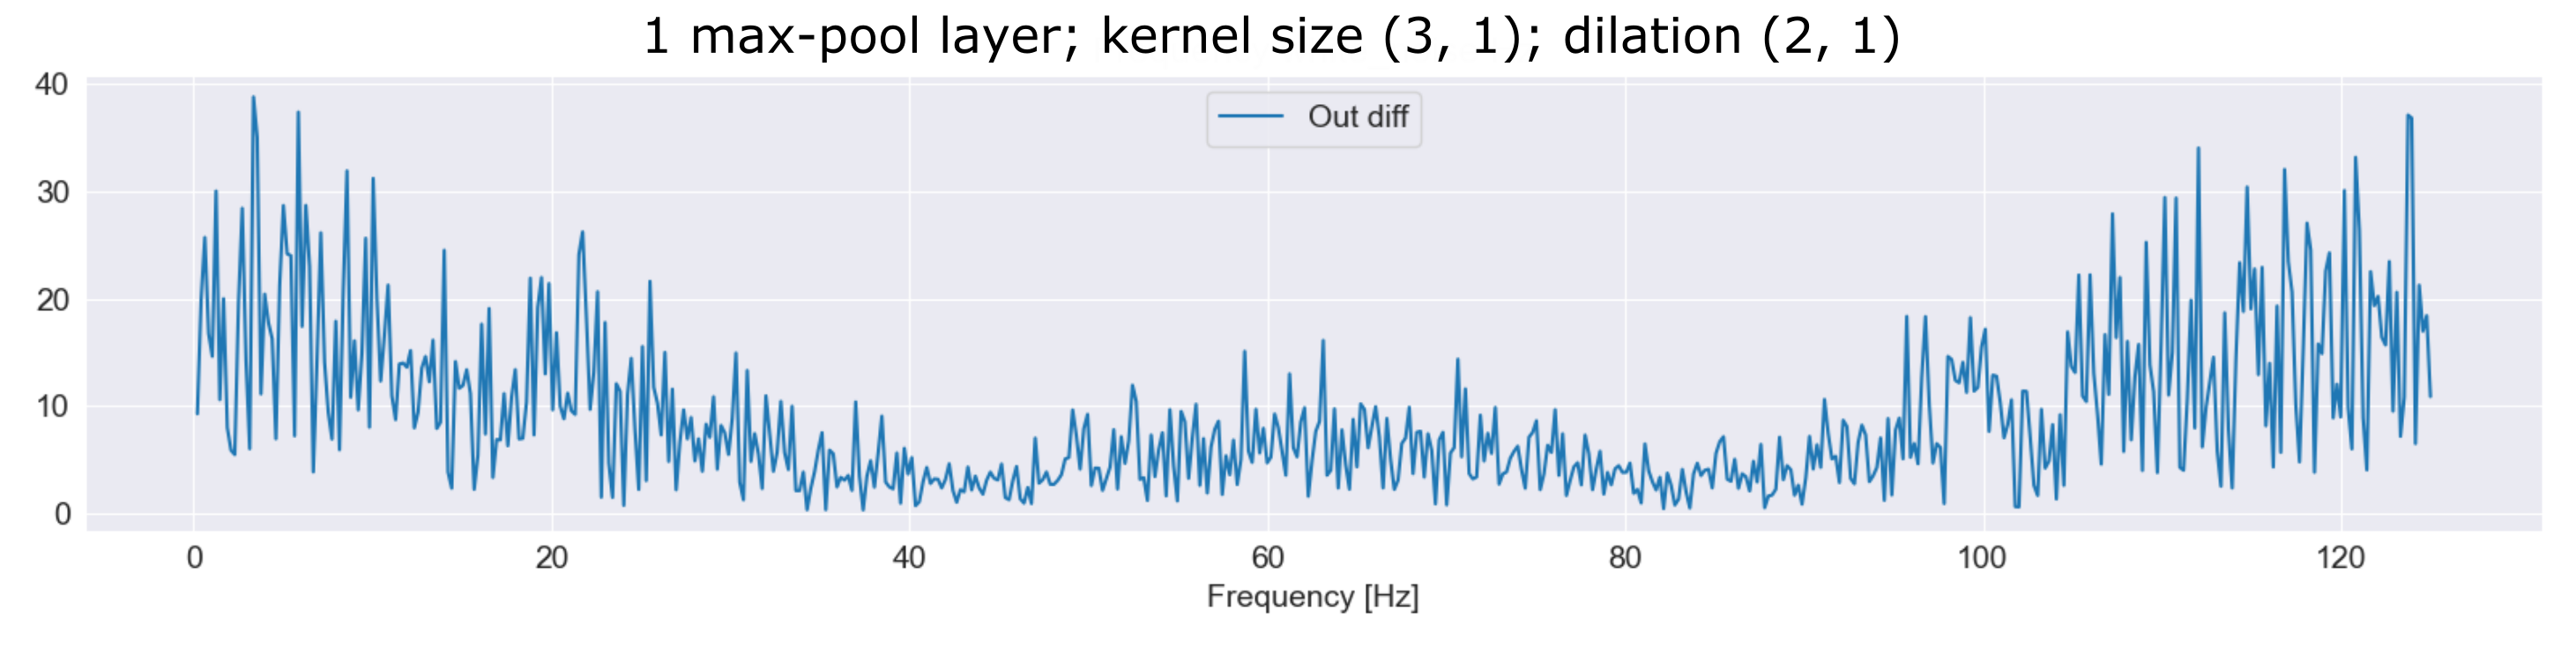
\includegraphics[width=1\linewidth]{img/ch4/absVel-maxpool-k3-d2}
   \caption{}
   \label{fig:maxpool-k3-d2}
\end{subfigure}

\caption[]{The blue line represents the difference between the output of a max-pool layer when original signal was given on input and when original signal with added white noise was given on input. The max-pool layer in \textbf{(a)} has dilation (3, 1) and kernel size (3, 1) and in \textbf{(b)} it has kernel size (3, 1) and dilation (2, 1).} 
\label{fig:max-pool-changes}
\end{figure}

The conclusions that can be made about the gradients peak when changing the kernel sizes and dilations of the max-pool layers are summarized below.
The majority of the above presented results suggests that the gradient peak is indeed an architecture artifact.
Its disappearance without loss of performance and the behaviour of the output signal when passed through single layers are in line with the hypothesis about frequency alignment.
The fact that the different kinds of channels (motor, non-motor) have similar gradient values at the peak also suggests that it only emerges because of the alignment.
If the motor channel gradients for the peak were visibly larger, it would support the hypothesis that some useful information is in this peak.
But because they are almost equal we can deduce that it is likely caused by the frequency alignment which should affect all channels in the same way.
The only argument speaking in favor of the gradient peak being informative for the network when making its decision is its amplification with training.
Nevertheless, this can be also attributed to the network not amplifying the peak but not actively working to suppress it as it occurs naturally due to the max-pool layers.
Lastly also the fact that the peak is visible only when the input window is shortened to give only one output diminishes the credibility of the peak containing information useful for decoding.
Without the averaging, the gradient method is less stable and therefore also less reliable.~\todo{Add citation\cite{}}
Overall, the gradient peak definitely cannot be taken as proof that the network is using high-gamma.
